\documentclass{standalone}
\usepackage{tikz}
\usetikzlibrary{patterns, positioning}
\usepackage[sfdefault]{ClearSans} %% option 'sfdefault' activates Clear Sans as the default text font
\usepackage[T1]{fontenc}

\begin{document}
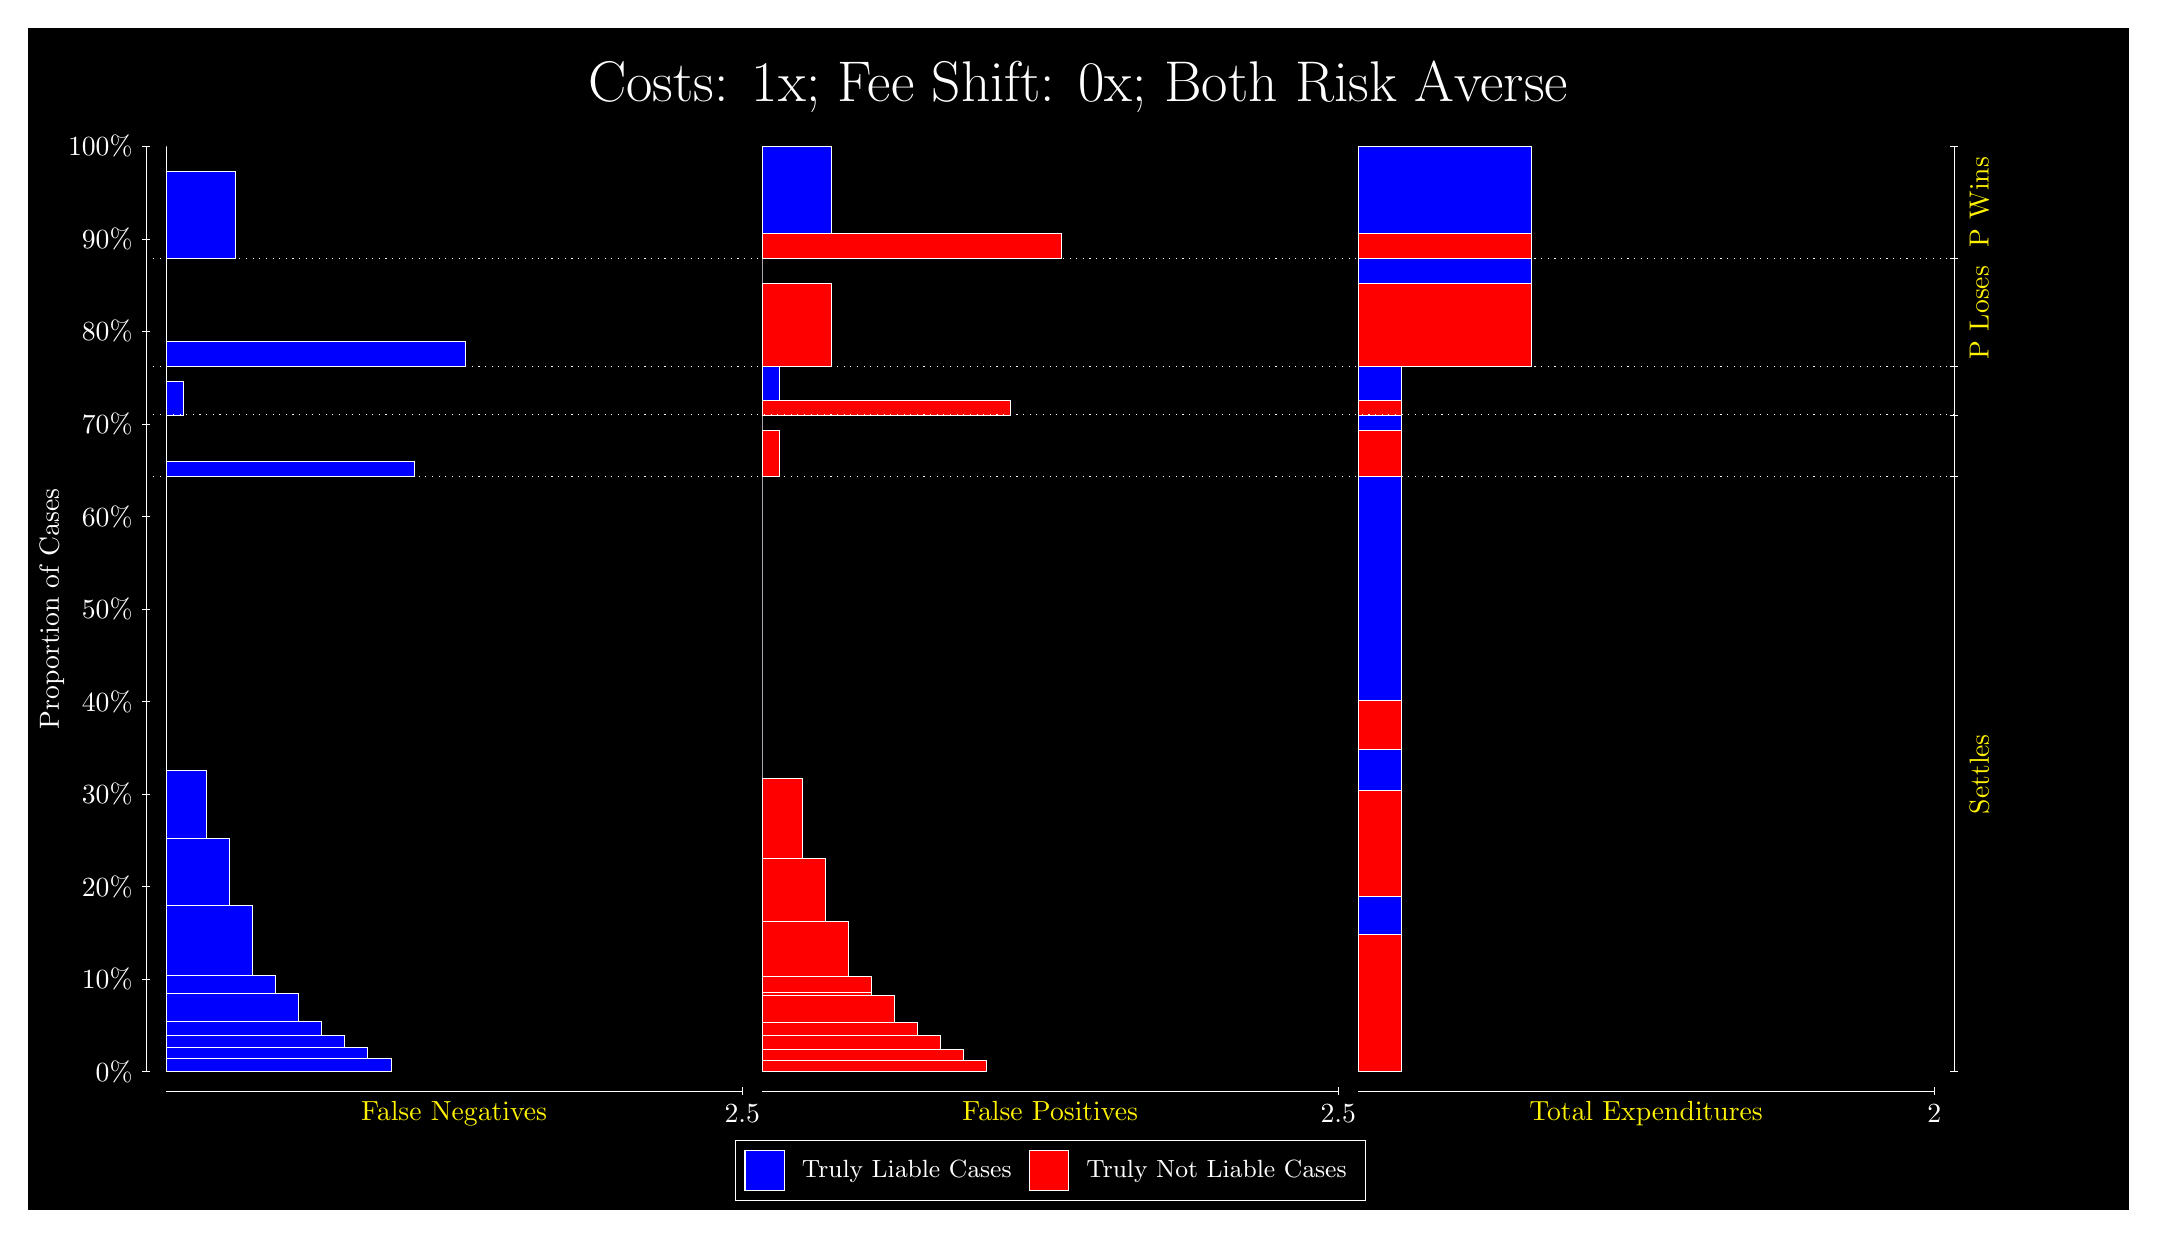
\begin{tikzpicture}
\draw[fill=black] (0,0) rectangle (26.667,15);
\draw[text=white] (0,13.5) rectangle (26.667,15) node[midway] {\huge Costs: 1x; Fee Shift: 0x; Both Risk Averse};
\draw[white, very thin] (1.5,1.75) -- (1.5,13.5);
\node[rotate=90, text=white, anchor=center] at (0.3, 7.625) {Proportion of Cases};
\draw[white, very thin] (1.45,1.75) -- (1.55,1.75);
\node[text=white, anchor=east] at (1.45, 1.75) {0\%};
\draw[white, very thin] (1.45,2.925) -- (1.55,2.925);
\node[text=white, anchor=east] at (1.45, 2.925) {10\%};
\draw[white, very thin] (1.45,4.1) -- (1.55,4.1);
\node[text=white, anchor=east] at (1.45, 4.1) {20\%};
\draw[white, very thin] (1.45,5.275) -- (1.55,5.275);
\node[text=white, anchor=east] at (1.45, 5.275) {30\%};
\draw[white, very thin] (1.45,6.45) -- (1.55,6.45);
\node[text=white, anchor=east] at (1.45, 6.45) {40\%};
\draw[white, very thin] (1.45,7.625) -- (1.55,7.625);
\node[text=white, anchor=east] at (1.45, 7.625) {50\%};
\draw[white, very thin] (1.45,8.8) -- (1.55,8.8);
\node[text=white, anchor=east] at (1.45, 8.8) {60\%};
\draw[white, very thin] (1.45,9.975) -- (1.55,9.975);
\node[text=white, anchor=east] at (1.45, 9.975) {70\%};
\draw[white, very thin] (1.45,11.15) -- (1.55,11.15);
\node[text=white, anchor=east] at (1.45, 11.15) {80\%};
\draw[white, very thin] (1.45,12.325) -- (1.55,12.325);
\node[text=white, anchor=east] at (1.45, 12.325) {90\%};
\draw[white, very thin] (1.45,13.5) -- (1.55,13.5);
\node[text=white, anchor=east] at (1.45, 13.5) {100\%};

\draw[white, very thin] (24.457,1.75) -- (24.457,13.5);
\draw[white, very thin] (24.407,1.75) -- (24.507,1.75);
\node[anchor=west] at (24.407, 1.75) {};
\draw[white, very thin] (24.407,9.3035) -- (24.507,9.3035);
\node[anchor=west] at (24.407, 9.3035) {};
\draw[white, very thin] (24.407,10.089) -- (24.507,10.089);
\node[anchor=west] at (24.407, 10.089) {};
\draw[white, very thin] (24.407,10.701) -- (24.507,10.701);
\node[anchor=west] at (24.407, 10.701) {};
\draw[white, very thin] (24.407,12.08) -- (24.507,12.08);
\node[anchor=west] at (24.407, 12.08) {};
\draw[white, very thin] (24.407,13.5) -- (24.507,13.5);
\node[anchor=west] at (24.407, 13.5) {};

\draw[white, very thin, fill=blue] (1.75,1.75) rectangle (4.6044,1.9217);
\draw[white, very thin, fill=blue] (1.75,1.9217) rectangle (4.3116,2.0518);
\draw[white, very thin, fill=blue] (1.75,2.0518) rectangle (4.0188,2.2071);
\draw[white, very thin, fill=blue] (1.75,2.2071) rectangle (3.7261,2.3922);
\draw[white, very thin, fill=blue] (1.75,2.3922) rectangle (3.4333,2.7426);
\draw[white, very thin, fill=blue] (1.75,2.7426) rectangle (3.1406,2.9692);
\draw[white, very thin, fill=blue] (1.75,2.9692) rectangle (2.8478,3.8553);
\draw[white, very thin, fill=blue] (1.75,3.8553) rectangle (2.5551,4.7108);
\draw[white, very thin, fill=blue] (1.75,4.7108) rectangle (2.2623,5.5757);
\draw[white, very thin, fill=red] (1.75,5.5757) rectangle (1.75,9.3035);
\draw[white, very thin, fill=blue] (1.75,9.3035) rectangle (4.8971,9.5054);
\draw[white, very thin, fill=red] (1.75,9.5054) rectangle (1.75,10.089);
\draw[white, very thin, fill=blue] (1.75,10.089) rectangle (1.9696,10.517);
\draw[white, very thin, fill=red] (1.75,10.517) rectangle (1.75,10.701);
\draw[white, very thin, fill=blue] (1.75,10.701) rectangle (5.5558,11.02);
\draw[white, very thin, fill=red] (1.75,11.02) rectangle (1.75,12.08);
\draw[white, very thin, fill=blue] (1.75,12.08) rectangle (2.6283,13.18);
\draw[white, very thin, fill=red] (1.75,13.18) rectangle (1.75,13.5);
\draw[white, very thin, fill=red] (9.3189,1.75) rectangle (12.173,1.8942);
\draw[white, very thin, fill=red] (9.3189,1.8942) rectangle (11.88,2.0286);
\draw[white, very thin, fill=red] (9.3189,2.0286) rectangle (11.588,2.2157);
\draw[white, very thin, fill=red] (9.3189,2.2157) rectangle (11.295,2.3763);
\draw[white, very thin, fill=red] (9.3189,2.3763) rectangle (11.002,2.7127);
\draw[white, very thin, fill=red] (9.3189,2.7127) rectangle (10.709,2.7503);
\draw[white, very thin, fill=red] (9.3189,2.7503) rectangle (10.709,2.9582);
\draw[white, very thin, fill=red] (9.3189,2.9582) rectangle (10.417,3.6544);
\draw[white, very thin, fill=red] (9.3189,3.6544) rectangle (10.124,4.4621);
\draw[white, very thin, fill=red] (9.3189,4.4621) rectangle (9.8312,5.4778);
\draw[white, very thin, fill=blue] (9.3189,5.4778) rectangle (9.3189,9.3035);
\draw[white, very thin, fill=red] (9.3189,9.3035) rectangle (9.5384,9.8876);
\draw[white, very thin, fill=blue] (9.3189,9.8876) rectangle (9.3189,10.089);
\draw[white, very thin, fill=red] (9.3189,10.089) rectangle (12.466,10.273);
\draw[white, very thin, fill=blue] (9.3189,10.273) rectangle (9.5384,10.701);
\draw[white, very thin, fill=red] (9.3189,10.701) rectangle (10.197,11.761);
\draw[white, very thin, fill=blue] (9.3189,11.761) rectangle (9.3189,12.08);
\draw[white, very thin, fill=red] (9.3189,12.08) rectangle (13.125,12.4);
\draw[white, very thin, fill=blue] (9.3189,12.4) rectangle (10.197,13.5);
\draw[white, very thin, fill=red] (16.888,1.75) rectangle (17.437,3.4994);
\draw[white, very thin, fill=blue] (16.888,3.4994) rectangle (17.437,3.9699);
\draw[white, very thin, fill=red] (16.888,3.9699) rectangle (17.437,5.3219);
\draw[white, very thin, fill=blue] (16.888,5.3219) rectangle (17.437,5.844);
\draw[white, very thin, fill=red] (16.888,5.844) rectangle (17.437,6.4704);
\draw[white, very thin, fill=blue] (16.888,6.4704) rectangle (17.437,9.3035);
\draw[white, very thin, fill=red] (16.888,9.3035) rectangle (17.437,9.8876);
\draw[white, very thin, fill=blue] (16.888,9.8876) rectangle (17.437,10.089);
\draw[white, very thin, fill=red] (16.888,10.089) rectangle (17.437,10.273);
\draw[white, very thin, fill=blue] (16.888,10.273) rectangle (17.437,10.701);
\draw[white, very thin, fill=red] (16.888,10.701) rectangle (19.083,11.761);
\draw[white, very thin, fill=blue] (16.888,11.761) rectangle (19.083,12.08);
\draw[white, very thin, fill=red] (16.888,12.08) rectangle (19.083,12.4);
\draw[white, very thin, fill=blue] (16.888,12.4) rectangle (19.083,13.5);
\draw[white, dotted] (1.5,9.3035) -- (24.457,9.3035);
\draw[white, dotted] (1.5,10.089) -- (24.457,10.089);
\draw[white, dotted] (1.5,10.701) -- (24.457,10.701);
\draw[white, dotted] (1.5,12.08) -- (24.457,12.08);
\draw[white, very thin] (1.75,1.5) -- (9.0689,1.5);
\node[text=yellow, anchor=north] at (5.4094, 1.5) {False Negatives};
\draw[white, very thin] (9.0689,1.45) -- (9.0689,1.55);
\node[text=white, anchor=north] at (9.0689, 1.45) {2.5};

\draw[white, very thin] (9.3189,1.5) -- (16.638,1.5);
\node[text=yellow, anchor=north] at (12.978, 1.5) {False Positives};
\draw[white, very thin] (16.638,1.45) -- (16.638,1.55);
\node[text=white, anchor=north] at (16.638, 1.45) {2.5};

\draw[white, very thin] (16.888,1.5) -- (24.207,1.5);
\node[text=yellow, anchor=north] at (20.547, 1.5) {Total Expenditures};
\draw[white, very thin] (24.207,1.45) -- (24.207,1.55);
\node[text=white, anchor=north] at (24.207, 1.45) {2};

\node[text=yellow, centered, rotate=90] at (24.777, 5.5268) {Settles};


\node[text=yellow, centered, rotate=90] at (24.777, 11.39) {P Loses};
\node[text=yellow, centered, rotate=90] at (24.777, 12.79) {P Wins};

\draw (12.978300999999998,1.5) node[draw=none] (baseCoordinate) {};
\begin{scope}[align=center]
        \matrix[scale=0.5, draw=white, below=0.5cm of baseCoordinate, nodes={draw}, column sep=0.1cm]{
            \node[rectangle, draw, minimum width=0.5cm, minimum height=0.5cm, fill=blue] {}; &
            \node[draw=none, font=\small, text=white] (B) {Truly Liable Cases}; &
            \node[rectangle, draw, minimum width=0.5cm, minimum height=0.5cm, fill=red] {}; &
            \node[draw=none, font=\small, text=white] (B) {Truly Not Liable Cases}; \\
            };
\end{scope}

\end{tikzpicture}
\end{document}